\PassOptionsToPackage{unicode=true}{hyperref} % options for packages loaded elsewhere
\PassOptionsToPackage{hyphens}{url}
%
\documentclass[12pt,]{article}
\usepackage{lmodern}
\usepackage{amssymb,amsmath}
\usepackage{ifxetex,ifluatex}
\usepackage{fixltx2e} % provides \textsubscript
\ifnum 0\ifxetex 1\fi\ifluatex 1\fi=0 % if pdftex
  \usepackage[T1]{fontenc}
  \usepackage[utf8]{inputenc}
  \usepackage{textcomp} % provides euro and other symbols
\else % if luatex or xelatex
  \usepackage{unicode-math}
  \defaultfontfeatures{Ligatures=TeX,Scale=MatchLowercase}
    \setmainfont[]{Times New Roman}
\fi
% use upquote if available, for straight quotes in verbatim environments
\IfFileExists{upquote.sty}{\usepackage{upquote}}{}
% use microtype if available
\IfFileExists{microtype.sty}{%
\usepackage[]{microtype}
\UseMicrotypeSet[protrusion]{basicmath} % disable protrusion for tt fonts
}{}
\IfFileExists{parskip.sty}{%
\usepackage{parskip}
}{% else
\setlength{\parindent}{0pt}
\setlength{\parskip}{6pt plus 2pt minus 1pt}
}
\usepackage{hyperref}
\hypersetup{
            pdftitle={Insert title of project here},
            pdfauthor={Name},
            pdfborder={0 0 0},
            breaklinks=true}
\urlstyle{same}  % don't use monospace font for urls
\usepackage[margin=2.54cm]{geometry}
\usepackage{longtable,booktabs}
% Fix footnotes in tables (requires footnote package)
\IfFileExists{footnote.sty}{\usepackage{footnote}\makesavenoteenv{longtable}}{}
\usepackage{graphicx,grffile}
\makeatletter
\def\maxwidth{\ifdim\Gin@nat@width>\linewidth\linewidth\else\Gin@nat@width\fi}
\def\maxheight{\ifdim\Gin@nat@height>\textheight\textheight\else\Gin@nat@height\fi}
\makeatother
% Scale images if necessary, so that they will not overflow the page
% margins by default, and it is still possible to overwrite the defaults
% using explicit options in \includegraphics[width, height, ...]{}
\setkeys{Gin}{width=\maxwidth,height=\maxheight,keepaspectratio}
\setlength{\emergencystretch}{3em}  % prevent overfull lines
\providecommand{\tightlist}{%
  \setlength{\itemsep}{0pt}\setlength{\parskip}{0pt}}
\setcounter{secnumdepth}{5}
% Redefines (sub)paragraphs to behave more like sections
\ifx\paragraph\undefined\else
\let\oldparagraph\paragraph
\renewcommand{\paragraph}[1]{\oldparagraph{#1}\mbox{}}
\fi
\ifx\subparagraph\undefined\else
\let\oldsubparagraph\subparagraph
\renewcommand{\subparagraph}[1]{\oldsubparagraph{#1}\mbox{}}
\fi

% set default figure placement to htbp
\makeatletter
\def\fps@figure{htbp}
\makeatother

\usepackage{etoolbox}
\makeatletter
\providecommand{\subtitle}[1]{% add subtitle to \maketitle
  \apptocmd{\@title}{\par {\large #1 \par}}{}{}
}
\makeatother

\title{Insert title of project here}
\providecommand{\subtitle}[1]{}
\subtitle{Web address for GitHub repository}
\author{Name}
\date{}

\begin{document}
\maketitle

\newpage
\tableofcontents 
\newpage
\listoftables 
\newpage
\listoffigures 
\newpage

\hypertarget{rationale-and-research-questions}{%
\section{Rationale and Research
Questions}\label{rationale-and-research-questions}}

In the United States, the National Ambient Air Quality Standards from
the 1970 Clean Air Act help monitor air pollutant levels. While
significant reductions in air pollution have been made since the
standards were put in place, there are still many areas that do not meet
the standards. California, in particular, has been cited as a leader in
air pollution, cities such as Los Angeles-Long Beach, Bakersfield and
Fresno-Madera having the highest recorded levels of ozone levels in the
country.

It is well established that exposure to higher levels of air pollutants
such as ozone (O3), nitrogen dioxide (NO2), and particulate matter
(PM2.5) is associated with reduced lung function, asthma exacerbations,
increased hospital visits, and death (Schraufnagel et al., 2019). In
fact, asthma is the leading chronic condition in children, affecting 1
in 12 children in the United States (Zahran, 2018). According to a
recent Center for Disease Control and Prevention (CDC) study, children
have higher rates of hospital and emergency department visits associated
with asthma compared to adults (Moorman et al., 2012). The health
impacts of asthma are not distributed equally among children, however.
Prevalence of asthma in children can differ by age, family history,
racial and ethnic group, and socioeconomic status (U.S. EPA, 2013).

As such, my study seeks to answer two main questions: * What are the
trends of O3, NO2 and PM2.5 in some of the most polluted cities in
California over a five-year period, from 2013 to 2017 ? * How is asthma
incidence in California impacted by O3 and PM2.5 levels, accounting for
socioeocnomic variables? Is this relationship different in children
compared to adults?

\newpage

\hypertarget{dataset-information}{%
\section{Dataset Information}\label{dataset-information}}

Provide information on how the dataset for this analysis were collected,
the data contained in the dataset, and any important pieces of
information that are relevant to your analyses. This section should
contain much of same information as the metadata file for the dataset
but formatted in a way that is more narrative.

Describe how you wrangled your dataset in a format similar to a methods
section of a journal article.

Add a table that summarizes your data structure (variables, units,
ranges and/or central tendencies, data source if multiple are used,
etc.). This table can be made in markdown text or inserted as a
\texttt{kable} function in an R chunk. If the latter, do not include the
code used to generate your table.

\hypertarget{epa-air-quality-datasets}{%
\subsection{EPA air quality datasets}\label{epa-air-quality-datasets}}

Air quality data were collected using EPA's Download Daily Data tool
(\url{https://www.epa.gov/outdoor-air-quality-data/download-daily-data}).

The following selections were made:

\begin{longtable}[]{@{}ll@{}}
\toprule
Option & Selection\tabularnewline
\midrule
\endhead
Pollutant & PM2.5, Ozone, and NO2\tabularnewline
Year & 2013-2017\tabularnewline
Geographic Area & California\tabularnewline
Download & Download CSV (spreadsheet)\tabularnewline
\bottomrule
\end{longtable}

The downloaded files, which were accessed on 2020-04-11, were saved in
the project folder path \texttt{./Data/Raw/Air\ quality/} as
\texttt{EPAair\_{[}Pollutant{]}\_CA\_{[}Year{]}\_raw.csv}. For example,
the O3 dataset for 2017 was saved as
\texttt{EPAair\_O3\_CA\_2017\_raw.csv}.

\hypertarget{pm2.5-dataset-content-information}{%
\subsubsection{PM2.5 dataset content
information}\label{pm2.5-dataset-content-information}}

This datset contains daily mean PM2.5 concentrations and the
corresponding air quality index (AQI) value in California over the years
2013-2017.

\begin{longtable}[]{@{}lll@{}}
\toprule
Year & Sites & Counties\tabularnewline
\midrule
\endhead
2013 & 149 & 52\tabularnewline
2014 & 152 & 52\tabularnewline
2015 & 151 & 52\tabularnewline
2016 & 151 & 52\tabularnewline
2017 & 152 & 51\tabularnewline
\bottomrule
\end{longtable}

\hypertarget{o3-dataset-content-information}{%
\subsubsection{O3 dataset content
information}\label{o3-dataset-content-information}}

This dataset contains daily maximum 8-hour O3 concentrations and the
corresponding air quality index (AQI) value in California over the years
2013-2017.

\begin{longtable}[]{@{}lll@{}}
\toprule
Year & Sites & Counties\tabularnewline
\midrule
\endhead
2013 & 183 & 49\tabularnewline
2014 & 182 & 49\tabularnewline
2015 & 182 & 49\tabularnewline
2016 & 182 & 49\tabularnewline
2017 & 181 & 49\tabularnewline
\bottomrule
\end{longtable}

\hypertarget{no2-dataset-content-information}{%
\subsubsection{NO2 dataset content
information}\label{no2-dataset-content-information}}

This dataset contains the daily maximum 1-hour NO2 concentration and the
corresponding air quality index (AQI) value in California over the years
2013-2017.

\begin{longtable}[]{@{}lll@{}}
\toprule
Year & Sites & Counties\tabularnewline
\midrule
\endhead
2013 & 102 & 33\tabularnewline
2014 & 105 & 33\tabularnewline
2015 & 108 & 33\tabularnewline
2016 & 109 & 33\tabularnewline
2017 & 106 & 33\tabularnewline
\bottomrule
\end{longtable}

All three datasets contain 20 variables (Table 2). Variable names
without descriptions are self-explanatory.

\begin{longtable}[]{@{}ll@{}}
\toprule
\begin{minipage}[b]{0.65\columnwidth}\raggedright
Variable\strut
\end{minipage} & \begin{minipage}[b]{0.29\columnwidth}\raggedright
Description\strut
\end{minipage}\tabularnewline
\midrule
\endhead
\begin{minipage}[t]{0.65\columnwidth}\raggedright
Date\strut
\end{minipage} & \begin{minipage}[t]{0.29\columnwidth}\raggedright
Month/day/year\strut
\end{minipage}\tabularnewline
\begin{minipage}[t]{0.65\columnwidth}\raggedright
Source\strut
\end{minipage} & \begin{minipage}[t]{0.29\columnwidth}\raggedright
AQS (Air Quality System) or AirNow\strut
\end{minipage}\tabularnewline
\begin{minipage}[t]{0.65\columnwidth}\raggedright
Site ID\strut
\end{minipage} & \begin{minipage}[t]{0.29\columnwidth}\raggedright
A unique number within the county identifying the site.\strut
\end{minipage}\tabularnewline
\begin{minipage}[t]{0.65\columnwidth}\raggedright
POC\strut
\end{minipage} & \begin{minipage}[t]{0.29\columnwidth}\raggedright
``Parameter Occurrence Code'' used to distinguish different instruments
that measure the same parameter at the same site.\strut
\end{minipage}\tabularnewline
\begin{minipage}[t]{0.65\columnwidth}\raggedright
Daily Mean PM2.5 Concentration\strut
\end{minipage} & \begin{minipage}[t]{0.29\columnwidth}\raggedright
\strut
\end{minipage}\tabularnewline
\begin{minipage}[t]{0.65\columnwidth}\raggedright
Daily Max 8-hour Ozone Concentration\strut
\end{minipage} & \begin{minipage}[t]{0.29\columnwidth}\raggedright
\strut
\end{minipage}\tabularnewline
\begin{minipage}[t]{0.65\columnwidth}\raggedright
Daily Max 1-hour NO2 Concentration\strut
\end{minipage} & \begin{minipage}[t]{0.29\columnwidth}\raggedright
\strut
\end{minipage}\tabularnewline
\begin{minipage}[t]{0.65\columnwidth}\raggedright
Units\strut
\end{minipage} & \begin{minipage}[t]{0.29\columnwidth}\raggedright
Units for concentration\strut
\end{minipage}\tabularnewline
\begin{minipage}[t]{0.65\columnwidth}\raggedright
Daily\_AQI\_VALUE\strut
\end{minipage} & \begin{minipage}[t]{0.29\columnwidth}\raggedright
Air quality index (range 0-500)\strut
\end{minipage}\tabularnewline
\begin{minipage}[t]{0.65\columnwidth}\raggedright
Site Name\strut
\end{minipage} & \begin{minipage}[t]{0.29\columnwidth}\raggedright
\strut
\end{minipage}\tabularnewline
\begin{minipage}[t]{0.65\columnwidth}\raggedright
DAILY\_OBS\_COUNT\strut
\end{minipage} & \begin{minipage}[t]{0.29\columnwidth}\raggedright
Number of observations per day\strut
\end{minipage}\tabularnewline
\begin{minipage}[t]{0.65\columnwidth}\raggedright
PERCENT\_COMPLETE\strut
\end{minipage} & \begin{minipage}[t]{0.29\columnwidth}\raggedright
\strut
\end{minipage}\tabularnewline
\begin{minipage}[t]{0.65\columnwidth}\raggedright
AQS\_PARAMETER\_CODE\strut
\end{minipage} & \begin{minipage}[t]{0.29\columnwidth}\raggedright
\strut
\end{minipage}\tabularnewline
\begin{minipage}[t]{0.65\columnwidth}\raggedright
AQS\_PARAMETER\_DESC\strut
\end{minipage} & \begin{minipage}[t]{0.29\columnwidth}\raggedright
\strut
\end{minipage}\tabularnewline
\begin{minipage}[t]{0.65\columnwidth}\raggedright
CBSA\_CODE\strut
\end{minipage} & \begin{minipage}[t]{0.29\columnwidth}\raggedright
\strut
\end{minipage}\tabularnewline
\begin{minipage}[t]{0.65\columnwidth}\raggedright
CBSA\_NAME\strut
\end{minipage} & \begin{minipage}[t]{0.29\columnwidth}\raggedright
\strut
\end{minipage}\tabularnewline
\begin{minipage}[t]{0.65\columnwidth}\raggedright
STATE\_CODE\strut
\end{minipage} & \begin{minipage}[t]{0.29\columnwidth}\raggedright
\strut
\end{minipage}\tabularnewline
\begin{minipage}[t]{0.65\columnwidth}\raggedright
STATE\strut
\end{minipage} & \begin{minipage}[t]{0.29\columnwidth}\raggedright
\strut
\end{minipage}\tabularnewline
\begin{minipage}[t]{0.65\columnwidth}\raggedright
COUNTY\_CODE\strut
\end{minipage} & \begin{minipage}[t]{0.29\columnwidth}\raggedright
\strut
\end{minipage}\tabularnewline
\begin{minipage}[t]{0.65\columnwidth}\raggedright
COUNTY\strut
\end{minipage} & \begin{minipage}[t]{0.29\columnwidth}\raggedright
\strut
\end{minipage}\tabularnewline
\begin{minipage}[t]{0.65\columnwidth}\raggedright
SITE\_LATITUDE\strut
\end{minipage} & \begin{minipage}[t]{0.29\columnwidth}\raggedright
\strut
\end{minipage}\tabularnewline
\begin{minipage}[t]{0.65\columnwidth}\raggedright
SITE\_LONGITUDE\strut
\end{minipage} & \begin{minipage}[t]{0.29\columnwidth}\raggedright
\strut
\end{minipage}\tabularnewline
\bottomrule
\end{longtable}

\hypertarget{data-wrangling}{%
\subsubsection{Data wrangling}\label{data-wrangling}}

Air quality datasets for different years were combined using
\texttt{rbind} to form one dataset for each pollutant.

The following columns were selected: * Date * Site.ID *
Daily.Max.1.hour.NO2.Concentration * DAILY\_AQI\_VALUE * Site.Name *
COUNTY

Additionally, columns for \texttt{Month} and \texttt{Year} were added
using the \texttt{Date} column.

\hypertarget{asthma-datasets}{%
\subsection{Asthma datasets}\label{asthma-datasets}}

Asthma data were collected using Tracking California's Asthma Data Query
tool (\url{https://trackingcalifornia.org/asthma/query}).

The following selections were made:

\begin{longtable}[]{@{}ll@{}}
\toprule
Option & Selection\tabularnewline
\midrule
\endhead
Type of Event & Emergency department visits due to asthma\tabularnewline
Age sub-group & Age 0-17, Age 18 \& over\tabularnewline
Year & 2013 - 2017\tabularnewline
How event is measured & Age-adjusted rates per 10,000\tabularnewline
Race/ethnicity & All Races/Ethnicities\tabularnewline
Gender/sex & Both Sexes\tabularnewline
Type of information & Conventional\tabularnewline
Type of geography & Zip codes\tabularnewline
\bottomrule
\end{longtable}

The downloaded files, which were accessed on 2020-04-12, were saved in
the project folder path \texttt{./Data/Raw/Asthma/} as
\texttt{TrackingCA\_Asthma\_ERVisits\_{[}Age\ Group{]}\_{[}Year{]}\_raw.csv}.
For example, the dataset for adults in 2013 was saved as
\texttt{TrackingCA\_Asthma\_ERVisits\_Adults\_2013\_raw.csv}.

\hypertarget{adult-asthma-dataset-content-information}{%
\subsubsection{Adult asthma dataset content
information}\label{adult-asthma-dataset-content-information}}

This dataset contains the annual rates of asthma-related ER visits for
adults in California over the years 2013-2017.

\hypertarget{children-asthma-dataset-content-information}{%
\subsubsection{Children asthma dataset content
information}\label{children-asthma-dataset-content-information}}

This dataset contains the annual rates of asthma-related ER visits for
children in California over the years 2013-2017.

Both datasets contain 2 variables. Variable names without descriptions
are self-explanatory.

\begin{longtable}[]{@{}ll@{}}
\toprule
\begin{minipage}[b]{0.47\columnwidth}\raggedright
Variable\strut
\end{minipage} & \begin{minipage}[b]{0.47\columnwidth}\raggedright
Description\strut
\end{minipage}\tabularnewline
\midrule
\endhead
\begin{minipage}[t]{0.47\columnwidth}\raggedright
Zip code\strut
\end{minipage} & \begin{minipage}[t]{0.47\columnwidth}\raggedright
\strut
\end{minipage}\tabularnewline
\begin{minipage}[t]{0.47\columnwidth}\raggedright
Incidence\strut
\end{minipage} & \begin{minipage}[t]{0.47\columnwidth}\raggedright
Age-adjusted rate of emergency department (ER) visits due to asthma per
10,000 California residents.\strut
\end{minipage}\tabularnewline
\bottomrule
\end{longtable}

\hypertarget{data-wrangling-1}{%
\subsubsection{Data wrangling}\label{data-wrangling-1}}

A `Year' column was added to all asthma datasets. Datasets for 2013-2017
were combined using \texttt{rbind} to form one dataset for each age
group (Adults, Children).

Since the asthma datasets provide only zip code information but not
county information, an online search was done to find zip codes and
their corresponding counties in California. This information was
datascraped into a data frame. This dataframe was then combined with the
adult dataset and the children dataset using \texttt{left\_join}. The
incidence rates were then grouped by county to calculate an average
incidence rate for each county.

Finally, adult and children asthma datasets were combined using
\texttt{full\_join}.

\hypertarget{demographics-dataset}{%
\subsection{Demographics dataset}\label{demographics-dataset}}

Demographic data were collected from County Health Rankings \& Roadmaps
(\url{https://www.countyhealthrankings.org/app/california/2019/downloads}).

Since demographics are assumed to remain somewhat constant over the
five-year period, only one dataset was chosen. The 2019 dataset, which
uses data published in 2017, was chosen.

The xls file, was accessed on 2020-04-12, was saved in the project
folder path \texttt{./Data/Raw/Demographics/} as
\texttt{CountyHealthRankings\_CA\_2019\_raw.xls}. Since there multiple
tabs in the xls file, relevant information from the file was taken and
converted into a csv file.The csv file was saved as
\texttt{CountyHealthRankings\_CA\_2019\_filtered\_raw.csv}

The following information is contained in the dataset: * FIPS * State *
County * Median Household Income * Population * \% African American * \%
Rural * \% Smokers * \% Uninsured

\newpage

\hypertarget{exploratory-analysis}{%
\section{Exploratory Analysis}\label{exploratory-analysis}}

Insert exploratory visualizations of your dataset. This may include, but
is not limited to, graphs illustrating the distributions of variables of
interest and/or maps of the spatial context of your dataset. Format your
R chunks so that graphs are displayed but code is not displayed.
Accompany these graphs with text sections that describe the
visualizations and provide context for further analyses.

Each figure should be accompanied by a caption, and each figure should
be referenced within the text.

Scope: think about what information someone might want to know about the
dataset before analyzing it statistically. How might you visualize this
information?

\hypertarget{air-quality-datasets}{%
\subsection{Air quality datasets}\label{air-quality-datasets}}

In examining the air quality index (AQI) values for the three pollutants
across all sites, there is not much temporal variation (Figure 1).
However, the frequency distrbution does differ depending on the
pollutant. NO2 generally has lower AQI values, which are aggregate well
below 50, the cut-off number for the ``Good'' air quality range. O3 and
PM2.5 have higher AQI values, which concentrated closer to 50, and also
contain more values that are above 50.

Among the four target sites--Bakersfield, Fresno, Los Angeles and San
Francisco--Bakersfield appears to have higher AQI values than the other
sites across all pollutants. In contrast, San Francisco generally has
lower AQI values compared to the other sites. Although AQI values for
NO2 stay below the ``Unhealthy'' range for all sites, the AQI values for
O3 and PM2.5 are generally in this range.

\begin{figure}
\centering
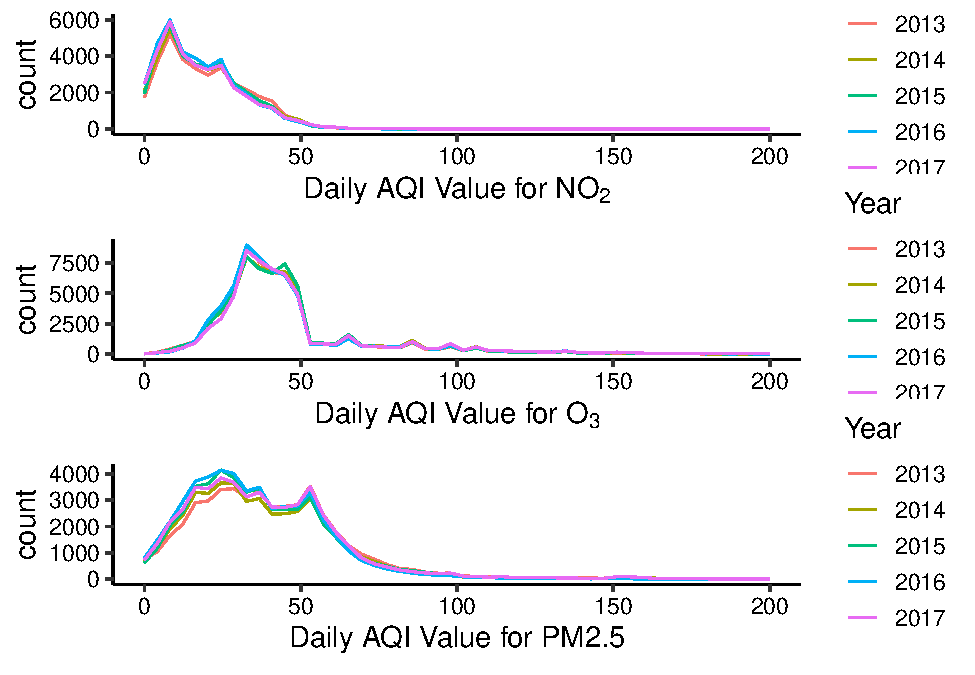
\includegraphics{Project_Template_files/figure-latex/unnamed-chunk-1-1.pdf}
\caption{Frequency plots of daily air quality index (AQI) values for the
three pollutants across the years 2013-2017.}
\end{figure}

\begin{figure}
\centering
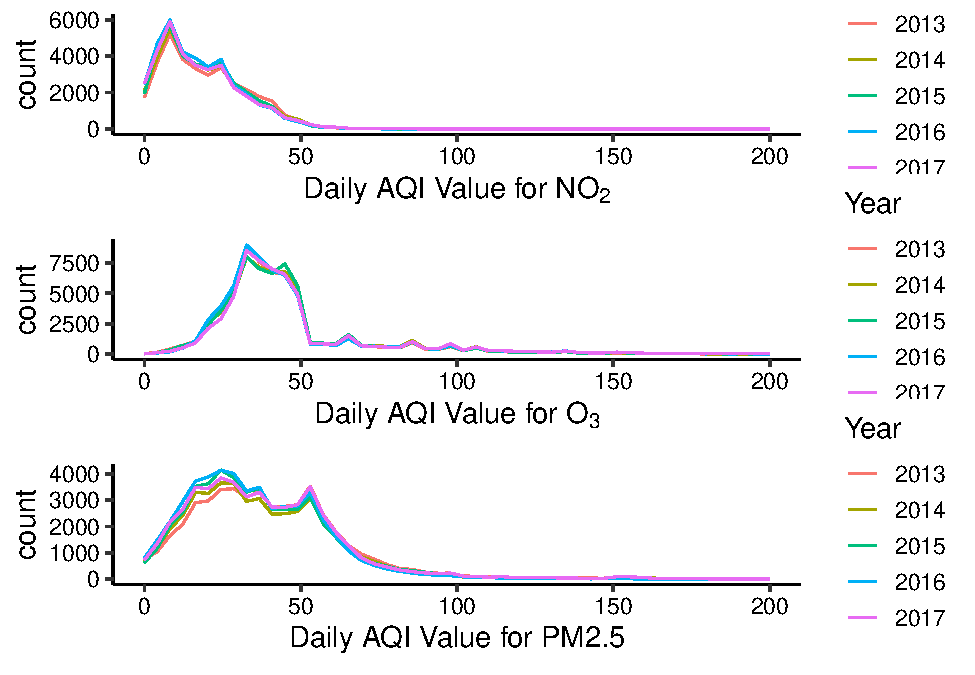
\includegraphics{Project_Template_files/figure-latex/unnamed-chunk-2-1.pdf}
\caption{Boxplots of daily air quality index (AQI) values for the three
pollutants in four key sites. The dashed line represents the lower bound
for the \texttt{Unhealthy\ (For\ sensitive\ groups)} range.}
\end{figure}

\newpage

\hypertarget{analysis}{%
\section{Analysis}\label{analysis}}

Insert visualizations and text describing your main analyses. Format
your R chunks so that graphs are displayed but code and other output is
not displayed. Instead, describe the results of any statistical tests in
the main text (e.g., ``Variable x was significantly different among y
groups (ANOVA; df = 300, F = 5.55, p \textless{} 0.0001)''). Each
paragraph, accompanied by one or more visualizations, should describe
the major findings and how they relate to the question and hypotheses.
Divide this section into subsections, one for each research question.

Each figure should be accompanied by a caption, and each figure should
be referenced within the text

\hypertarget{question-1-insert-specific-question-here-and-add-additional-subsections-for-additional-questions-below-if-needed}{%
\subsection{Question 1: \textless{}insert specific question here and add
additional subsections for additional questions below, if
needed\textgreater{}}\label{question-1-insert-specific-question-here-and-add-additional-subsections-for-additional-questions-below-if-needed}}

\hypertarget{question-2}{%
\subsection{Question 2:}\label{question-2}}

\newpage

\hypertarget{summary-and-conclusions}{%
\section{Summary and Conclusions}\label{summary-and-conclusions}}

Summarize your major findings from your analyses in a few paragraphs.
What conclusions do you draw from your findings? Relate your findings
back to the original research questions and rationale.

\newpage

\hypertarget{references}{%
\section{References}\label{references}}

\textless{}add references here if relevant, otherwise delete this
section\textgreater{}

\end{document}
